% !TeX spellcheck = es_ES
%%%%%%%%%%%%%%%%%%%%%%%%%%%%%%%%%%%%%%%%%%%%%%%%%%
% Plantilla presentación Beamer no oficial - Universidad Nacional de Colombia
%%%%%%%%%%%%%%%%%%%%%%%%%%%%%%%%%%%%%%%%%%%%%%%%%%
%------------------
% LICENCIA
%------------------
% Copyright (c) 2023 by Fabio Calderón
%
% This work is licensed under the Creative Commons Attribution 4.0 International License. (CC BY-NC-SA 4.0)
%
% To view a copy of this license, visit ``http://creativecommons.org/licenses/by-nc-sa/4.0/'' or send a letter to Creative Commons, PO Box 1866, Mountain View, CA 94042, USA.
%------------------
% IMPORTANTE: Leer todas las intrucciones (en formato de comentarios) en cada archivo de esta plantilla.
%
% Esta plantilla se ha desarrollado siguiendo las guías de identidad de la Universidad Nacional de Colombia (https://identidad.unal.edu.co/).
%------------------
% REQUERIMIENTOS
%------------------
% El inicio del documento con "\documentclass[aspectratio=169,usenames,dvipsnames]{beamer}" es obligatiorio, pues la plantilla ha sido desarrollada para el tamaño 16:9 y requiere los paquetes "xcolor" y "tikz".
%------------------
% CRÉDITOS
%------------------
% Esta plantilla es una adaptación del archivo público "University of Udine Unofficial Beamer Theme" por Marco Basaldella (Creative Commons CC BY 4.0). Disponible en: https://www.overleaf.com/latex/templates/university-of-udine-unofficial-beamer-theme/zndkgxrjsdzt.
%
% También se han tomado elementos de "Leiden University Beamer Theme" por J.P. van Leenen (LaTeX Project Public License 1.3c). Disponible en: https://www.overleaf.com/latex/templates/leiden-university-beamer-theme/ryfcpypnvzhr.
%
% Crédito de imágenes usadas:
% - Portada: "Skyscrapers in Bogota's downtown" por Mayor's Office of Bogota. https://commons.wikimedia.org/wiki/File:Bogota_Skyline.jpg. CC BY-SA 4.0.
% - framepic background: "	Biblioteca Ernesto Guhl, Ciudad Universitaria, Universidad Nacional de Colombia" por Rubashkyn. https://commons.wikimedia.org/wiki/File:Biblioteca_Ernesto_Guhl,_Universidad_Nacional,_Bogot%C3%A1.JPG. GFDL.
% - Logos UNAL: identidad.unal.edu.co.
%------------------
% ACERCA DEL AUTOR
%------------------
% Desarollado por Fabio Calderón en su cuarto y último año del Doctorado en Ciencias-Matemáticas de la Universidad Nacional de Colombia.
% Sugerencias/Comentarios: facalderonm@unal.edu.co
%------------------
% TODO
%------------------
% - Fix warnings of overfull at frames with title.
%%%%%%%%%%%%%%%%%%%%%%%%%%%%%%%%%%%%%%%%%%%%%%%%%%
%------------------
% DOCUMENT TYPE
%------------------
\documentclass[aspectratio=169,usenames,dvipsnames,spanish]{beamer}
% Replace "spanish" for "english" or any other language.
%%%%%%%%%%%%%%%%%%%%%%%%%%%%%%%%%%%%%%%%%%%%%%%%%%
%------------------
% DOCUMENT THEME
%------------------
\usetheme{UNAL}
%%%%%%%%%%%%%%%%%%%%%%%%%%%%%%%%%%%%%%%%%%%%%%%%%%
%------------------
% PACKAGES
%------------------
\usepackage{graphics,graphicx} % To insert graphs. They must be in the same folder than the .TEX file.
\usepackage{amsthm, amssymb, amsfonts, latexsym, mathtools,thmtools,bbm} % Enviroments and several math symbols.
\usepackage{ragged2e} % Justifies text.
%\usepackage[swedish]{babel}
%\usepackage[T1]{fontenc}
%\usepackage[latin1]{inputenc}
\usepackage{tikzsymbols} % Emojis.
\usepackage{comment} % To comment huge portions of text.
\usepackage{multicol} % For multiple columns of text or listings.
\usepackage{verbatim} % Para código.
\usepackage{bm}
% Agregar aquí los paquetes adicionales que se necesiten.
%%%%%%%%%%%%%%%%%%%%%%%%%%%%%%%%%%%%%%%%%%%%%%%%%%
%------------------
% INFO
%------------------
\title[First Lab. Linear Control Theory]{First Lab. Linear Control Theory}
\subtitle{Canonical Realizations and Electronic Design}
\vspace{-0.5cm}
\author[Valeria Orozco]{Valeria Orozco}
\institute{Facultad de Ingenieria - Universidad Tecnologica de Pereira}
\vspace{0.3cm}
\date{\today}
% IMPORTANTE: Si alguno de los parámetros es muy largo para la portada o se requieren varias líneas (ejemplo: varios autores), en el archivo
%%%%%%%%%%%%%%%%%%%%%%%%%%%%%%%%%%%%%%%%%%%%%%%%%%
%%%%%%%%%%%%%%%%%%%%%%%%%%%%%%%%%%%%%%%%%%%%%%%%%%
%%%%%%%%%%%%%%%%%%%%%%%%%%%%%%%%%%%%%%%%%%%%%%%%%%
\begin{document}
\justifying %Este comando justifica todo el texto FUERA de cajas/enviroments. Para también justificar el texto en cajas/enviroments, se debe usar este mismo comando dentro de la caja/enviroment, justo antes del texto.
%------------------
% PORTADA
%------------------
\begin{frame}
    \titlepage 
    % La imagen de fondo, su opacidad y posición se pueden modificar en beamerinnerthemeUNAL.sty.
\end{frame}
%------------------
% TABLA DE CONTENIDOS
%------------------
\begin{frame}{Contenidos} %English: Outline
    \tableofcontents
\end{frame}
\section{Canonical Controller Realization}
\begin{frame}{Canonical Controller Realization}
\begin{columns}[c]
		\column{.5\textwidth}  
       
		\column{.5\textwidth} % Right column and width
	\end{columns}
     \begin{figure}[h]
		\centering
		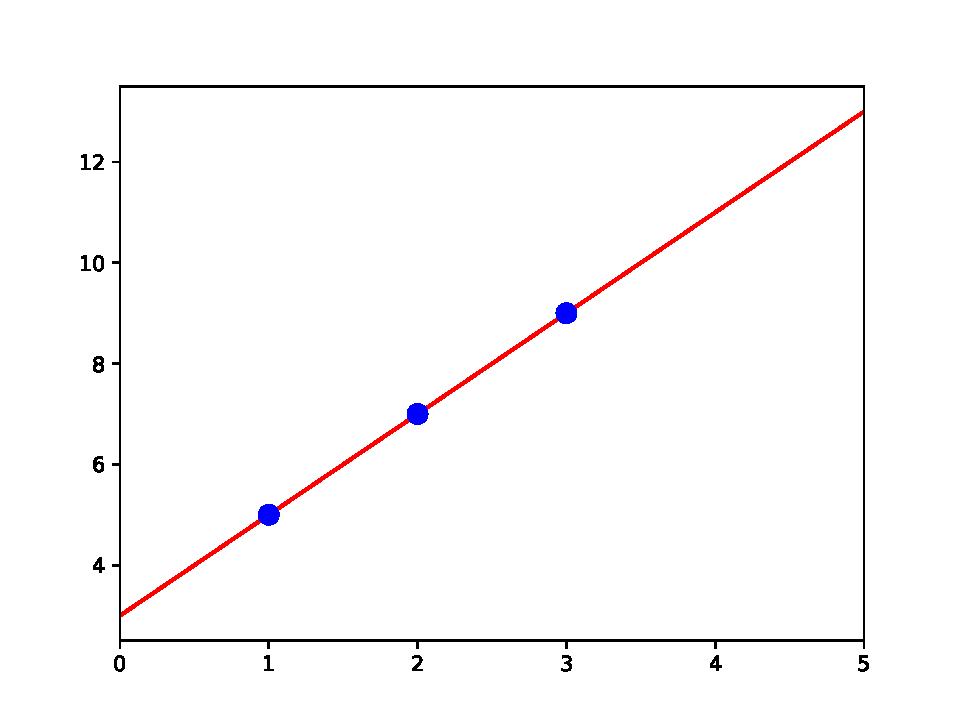
\includegraphics[width=0.25\textwidth]{slides_pic_1.pdf}
	\end{figure}
     Canonical Controller Realization:
        \begin{align}
        \left(\begin{array}{c}\dot{x}_{1}(t)
        \\
        \dot{x}_{2}(t)
        \\
        \dot{x}_{3}(t)\end{array}\right)=\left(\begin{array}{ccc}
        -11&-39&-29
        \\
        1&0&0
        \\
        0&1&0
        \end{array}\right)
        \left(\begin{array}{c}x_{1}(t)
        \\
        x_{2}(t)
        \\
        x_{3}(t)\end{array}\right)
        +\left(\begin{array}{c}1
        \\
        0
        \\
        0\end{array}\right)u(t)
        \end{align}
\end{frame}
\begin{frame}{Canonical Controller Realization}
\begin{columns}[c]
		\column{.5\textwidth}  
       \begin{figure}[h]
		\centering
		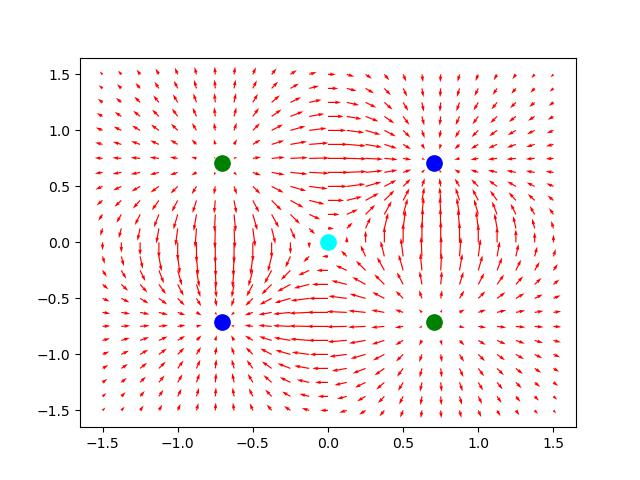
\includegraphics[width=0.75\textwidth]{Gaussian_Vector_Field.jpg}
	\end{figure}
		\column{.5\textwidth} % Right column and width
        \begin{figure}[h]
		\centering
		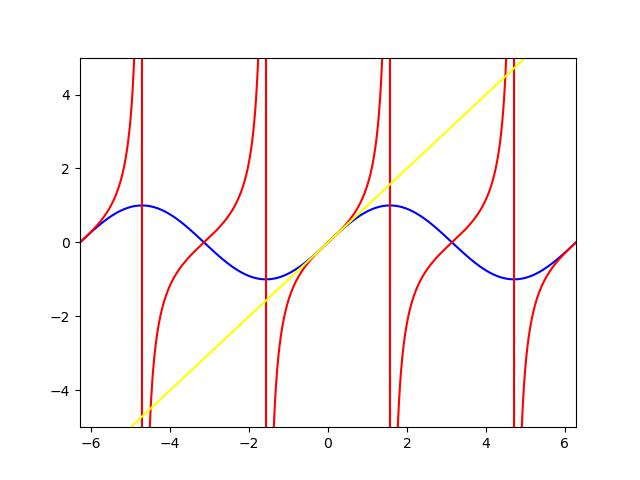
\includegraphics[width=0.75\textwidth]{Approximation_1.jpg}
	\end{figure}
	\end{columns}
\end{frame}
\section{Least Squares Equations}
\begin{frame}{Least Squares Equations}
Model for Linear Regression parameters:
$$
\left(\begin{array}{cc}
\sum_{m=1}^{N}x_{m}^{2}&\sum_{m=1}^{N}x_{m}
\\
\sum_{m=1}^{N}x_{m}&N
\end{array}\right)\left(\begin{array}{c}
a
\\
b
\end{array}\right)
=\left(\begin{array}{c}
\sum_{m=1}^{N}x_{m}y_{m}
\\
\sum_{m=1}^{N}y_{m}
\end{array}\right)
$$
Which yields the following least squares solution:
$$
a=\frac{N\sum_{m=1}^{N}x_{m}y_{m}-\sum_{m=1}^{N}x_{m}\sum_{m=1}^{N}y_{m}}{N\sum_{m=1}^{3}x_{m}^{2}-\left(\sum_{m=1}^{N}x_{m}\right)^{2}}
$$
$$
b=\frac{\sum_{m=1}^{N}x_{m}^{2}\sum_{m=1}^{N}y_{m}-\sum_{m=1}^{N}x_{m}\sum_{m=1}^{N}x_{m}y_{m}}{N\sum_{m=1}^{3}x_{m}^{2}-\left(\sum_{m=1}^{N}x_{m}\right)^{2}}
$$
\end{frame}
\section{Comparissions}
\subsection{Compare Exact vs Approximate}
\begin{frame}{Degree of Doctor of Philosophy (PhD)}
\begin{columns}[c]
		\column{.5\textwidth}   
		\begin{figure}[h]
		\centering
		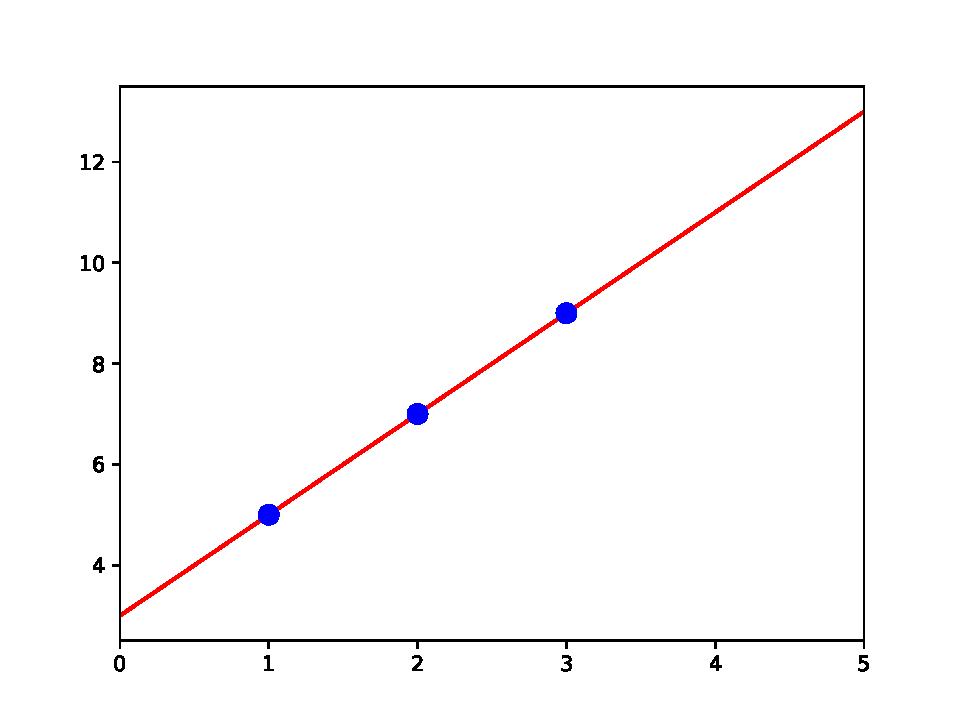
\includegraphics[width=1.0\textwidth]{slides_pic_1.pdf}
	\end{figure}
		\column{.5\textwidth} % Right column and width
        \vspace{-0.5cm}
        \begin{figure}[h]
		\centering
		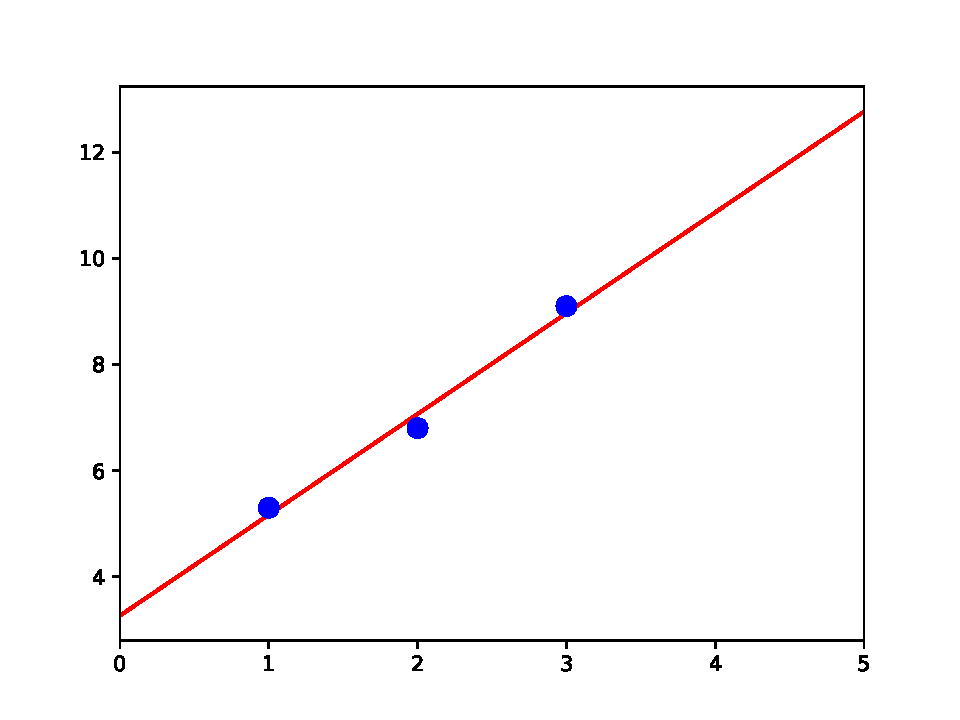
\includegraphics[width=1.0\textwidth]{slides_pic_2.pdf}
	\end{figure}
	\end{columns}
\end{frame}
\begin{frame}{Quadratic Regression Models}
\begin{columns}[c]
		\column{.5\textwidth}   
Consider the square mean error of a quadratic regression model given by:
		\column{.5\textwidth} % Right column and width
        
		
        

	\end{columns}
\end{frame}
\section{Conclusions}
\begin{frame}{Conclusions}
\begin{columns}[c]
		\column{.5\textwidth}   
     \begin{enumerate}
         \item \color{red} We observed the Dynamic Evolution of the Physical System Realized in Controller Canonical Form.
     \end{enumerate}
		\column{.5\textwidth} % Right column and width
        \begin{itemize}
            \item \color{blue} Here we considered non-inverter integrators (Miller Integrators)
        \end{itemize}
	\end{columns}
\end{frame}
\end{document}
%%%%%%%%%%%%%%%%%%%%%%%%%%%%%%%%%%%%%%%%%%%%%%%%%%
%%%%%%%%%%%%%%%%%%%%%%%%%%%%%%%%%%%%%%%%%%%%%%%%%%
%%%%%%%%%%%%%%%%%%%%%%%%%%%%%%%%%%%%%%%%%%%%%%%%%%